\documentclass[10pt,letterpaper]{article}
\usepackage[utf8]{inputenc}
\usepackage{amsmath}
\usepackage{amsfonts}
\usepackage{amssymb}
\usepackage{graphicx}

\usepackage{tikz}
\usetikzlibrary{arrows.meta}

\tikzset{every picture/.style={/utils/exec={\sffamily}}}

\begin{document}

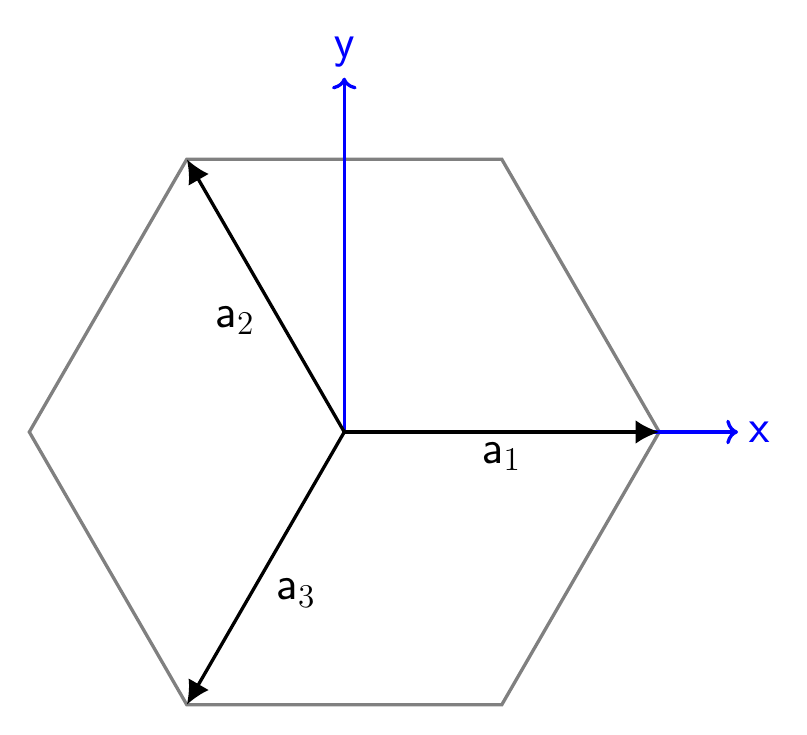
\begin{tikzpicture}[scale=2.0]

%Basal plane view
\draw[gray, very thick] (2,0) -- (1, {sqrt(3)}) -- (-1, {sqrt(3)}) -- (-2,0) -- (-1, -{sqrt(3)}) -- (1, -{sqrt(3)}) -- (2,0);

% Add the Cartesian axes
\draw[blue, very thick, ->] (0,0) -- (2.5,0) node [right] {\LARGE x};
\draw[blue, very thick, ->] (0,0) -- (0,2.25) node [above] {\LARGE y};

%Add the Miller-Bravis axes
\draw[very thick, -{Latex[length=3mm,width=3mm]}] (0,0) -- (2,0) node [midway, below] {\LARGE a$_1$};
\draw[very thick, -{Latex[length=3mm,width=3mm]}] (0,0) -- (-1, {sqrt(3)}) node [midway, below left] {\LARGE a$_2$};
\draw[very thick, -{Latex[length=3mm,width=3mm]}] (0,0) -- (-1, -{sqrt(3)}) node [midway, below right] {\LARGE a$_3$};

\end{tikzpicture}

\end{document}
